\subsection{Laser VCSEL 980\,nm --- omówienie wyników}
Pomiar przeprawadzany był w temperaturach chłodnicy od 283\,K do 363\,K, krokiem co 5\,K. Wartości wyznaczonego prądu progowego
znajdują się w tabeli~\ref{tab:tabela_vcsel850}. Rysunki od ~\ref{fig:plot_fit_i_th4_980} do ~\ref{fig:plot_eff_via_current_all_980} dotyczą lasera
VCSEL 980\,nm.
\begin{itemize}
\item Wykres na rysunku~\ref{fig:plot_fit_i_th4_980} przedstawia sposób wyznaczana wartość prądu progowego. Następnie na podstawie
wyznaczonych wartości w danej temperaturze, sporządziłem wykres prądu progowego w zależności od temperatury
przedstawiony na rysunku~\ref{fig:plot_temp_i_th_log_lin_980}. Jak widzimy wykres ten charakteryzuje się pewnym prądem
minimalnym osiągniętym w temperaturze 288\,K.
\item Analizując wykres napięcia na laserze od prądu wejściowego przedstawiony na rysunku~\ref{fig:plot_i_v_i_l_980}
można zauważyć, że wraz ze wzrostem temperatury na chłodnicy
maleje opór lasera. Także, wraz z wyższą temperaturą chłodnicy maleje moc wyjściowa lasera.
\item Wykres na rysunku~\ref{fig:plot_eff_via_current4_980} przedstawia sprawność różniczkowa lasera w funkcji prądu wejściowego
od temperatury na chłodnicy. W górnej części rysunku pokazana jest zależność mocy wyjściowej od prądu, do której dopasowałem
funkcją kwadratowa dla punktów leżących powyżej wartości prądu progowego. Dopasowana funkcja zbliżona jest do funkcji kwadratowej,
przez co zmiany sprawności wraz z wzrostem prądu jest dosyć duża.
\item Wykres na rysunku~\ref{fig:plot_eff_via_current_all_980} przedstawia jak zmienia się sprawność lasera od temperatury chłodnicy.
Funkcje, które przedstawiają sprawność zostały wyznaczone analogicznie jak te przedstawione na rysunku~\ref{fig:plot_eff_via_current4_980}.
Analizując ten wykres, dochodzę do wniosku, że wraz z wyższą temperaturą sprawność lasera maleje.
\end{itemize}
\begin{table}
\begin{center}
\caption{ Wyznaczone wartośc prądu progowego $I_{\mathrm{th}}$ w różnych temperaturach $T$ dla lasera VCSEL 980\,nm.}
\begin{tabular}{ | C{1.5cm}|  C{3.0cm} | C{1.5cm} | C{3.0cm}| C{1.5cm} | C{3.0cm}|}
\hline
$T$ [K] &   $I_{\mathrm{th}}$ [mA]  &  $T$ [K] &   $I_{\mathrm{th}}$ [mA]  &  $T$ [K] &   $I_{\mathrm{th}}$ [mA] 	\\ \hline
283      &   1.0 $\pm$ 0.04  & 288      &   0.94 $\pm$ 0.03       & 293		 &   0.98 $\pm$ 0.03  \\ \hline
298		 &   1.05 $\pm$ 0.04  & 303		 &   1.1 $\pm$ 0.03  & 308		 &   1.18 $\pm$ 0.03  \\ \hline
313		 &   1.23 $\pm$ 0.03  & 318		 &   1.25 $\pm$ 0.03  & 323		 &   1.36 $\pm$ 0.04  \\ \hline
328		 &   1.47 $\pm$ 0.03  & 333		 &   1.59 $\pm$ 0.04    & 338		 &   1.63 $\pm$ 0.04  \\ \hline
343		 &   1.76 $\pm$ 0.04    & 348		 &   1.86 $\pm$ 0.06    & 353		 &   2.07 $\pm$ 0.05  \\ \hline
358      &   2.25 $\pm$ 0.06  & 363 & 2.48 $\pm$ 0.06 \\ \cline{1-4}
\end{tabular}
\end{center}
\end{table}
\begin{figure}
\center
  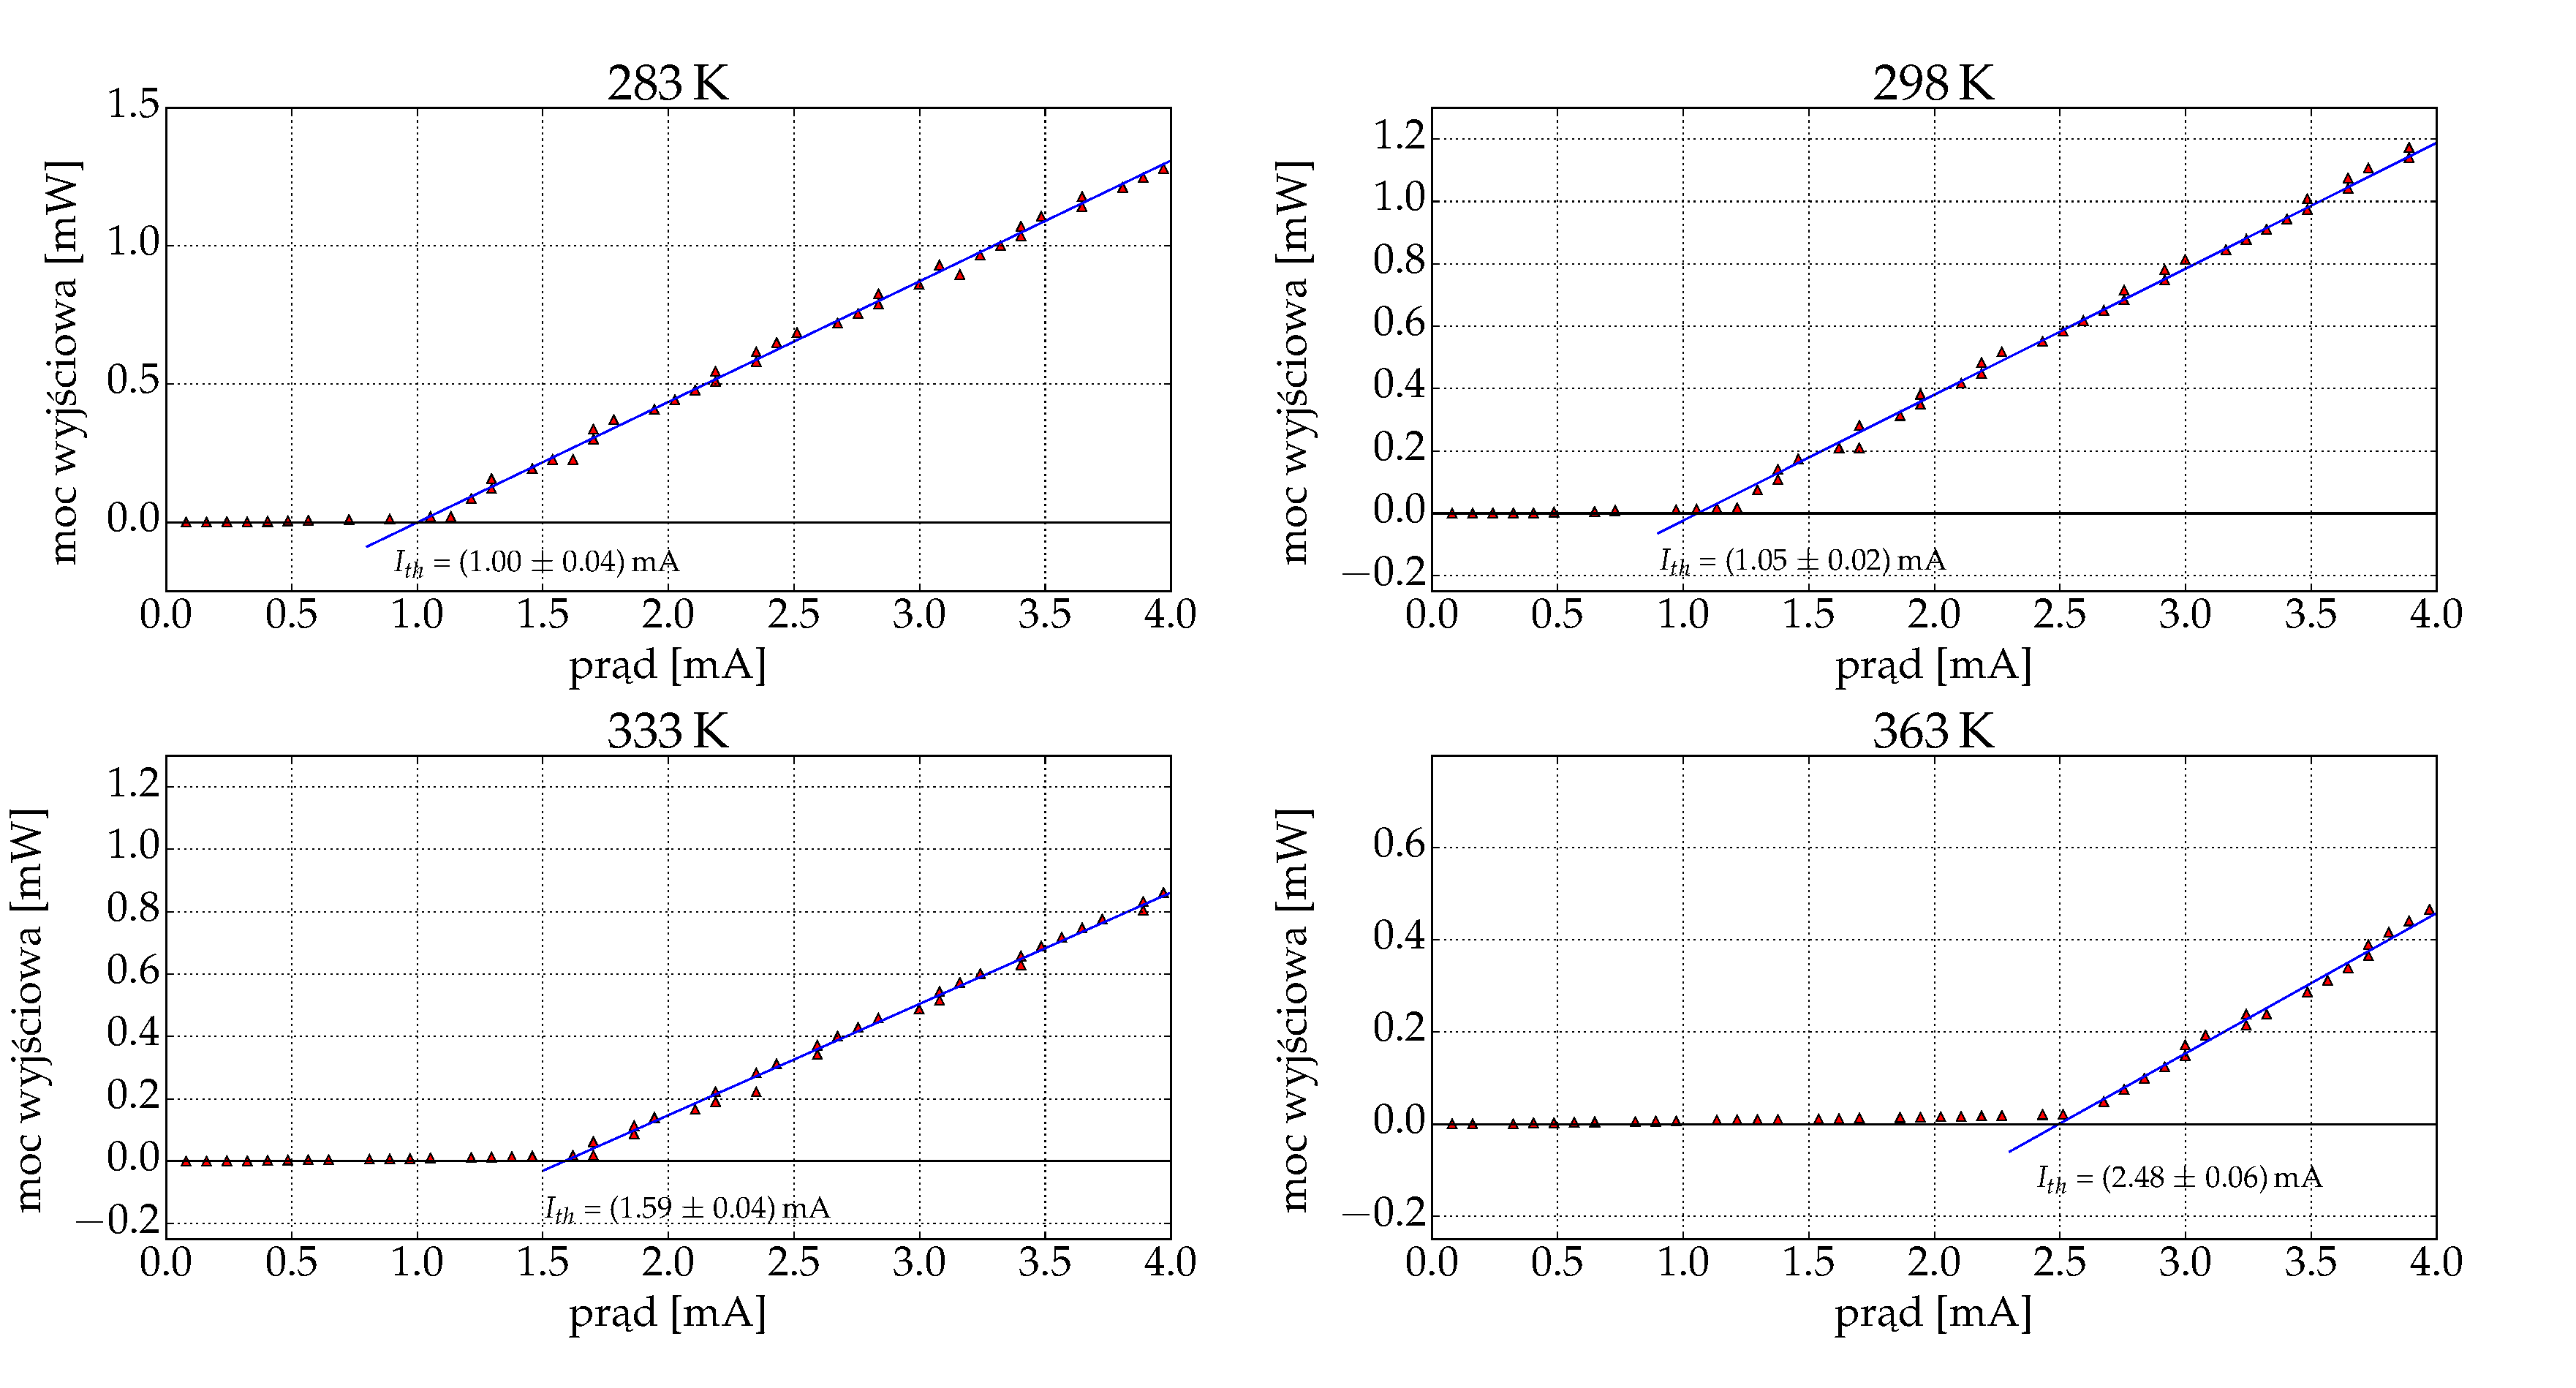
\includegraphics[scale=0.30]{plot980/plot_fit_i_th4.eps}
  \caption{Wykres ilustrujący wyznaczanie prądu progow dla lasera VCSEL 980\,nm.}
  \label{fig:plot_fit_i_th4_980}
\end{figure}
\begin{figure}
\center
  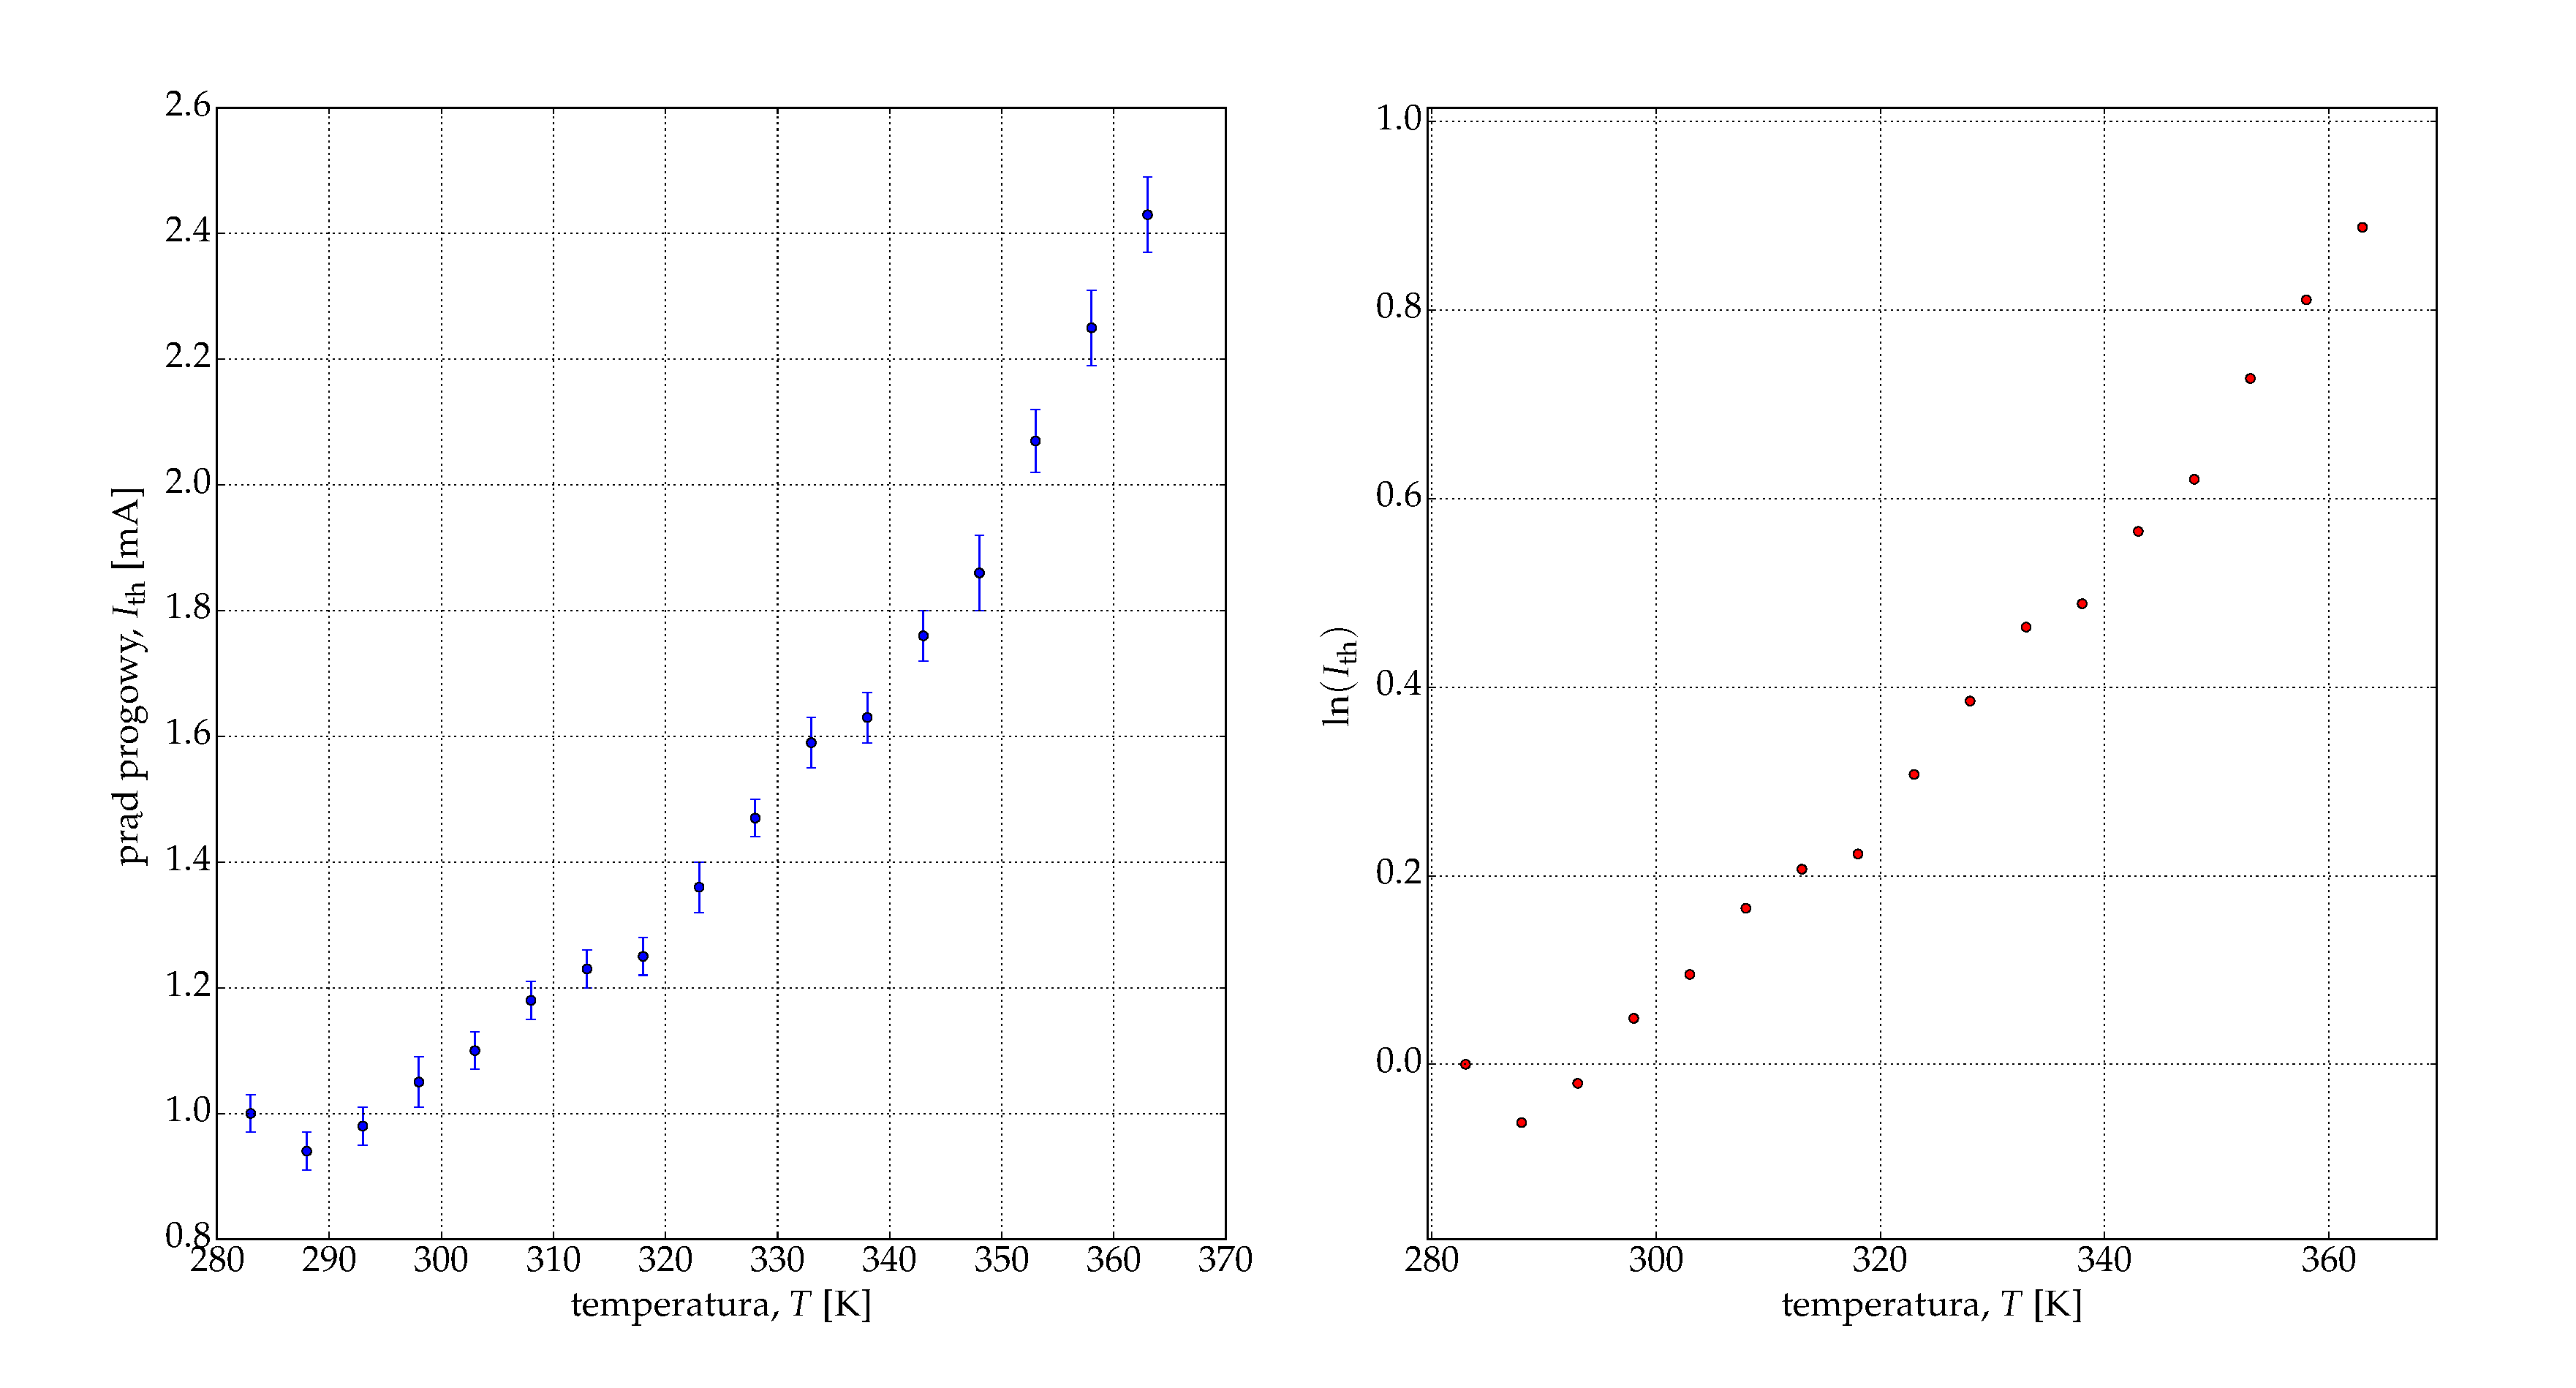
\includegraphics[scale=0.30]{plot980/plot_temp_i_th_log_lin.eps}
  \caption{Wykres prądu progow od temperatury dla lasera VCSEL 980\,nm w skali liniowej oraz logarytmicznej.}
  \label{fig:plot_temp_i_th_log_lin_980}
\end{figure}
\begin{figure}
\center
  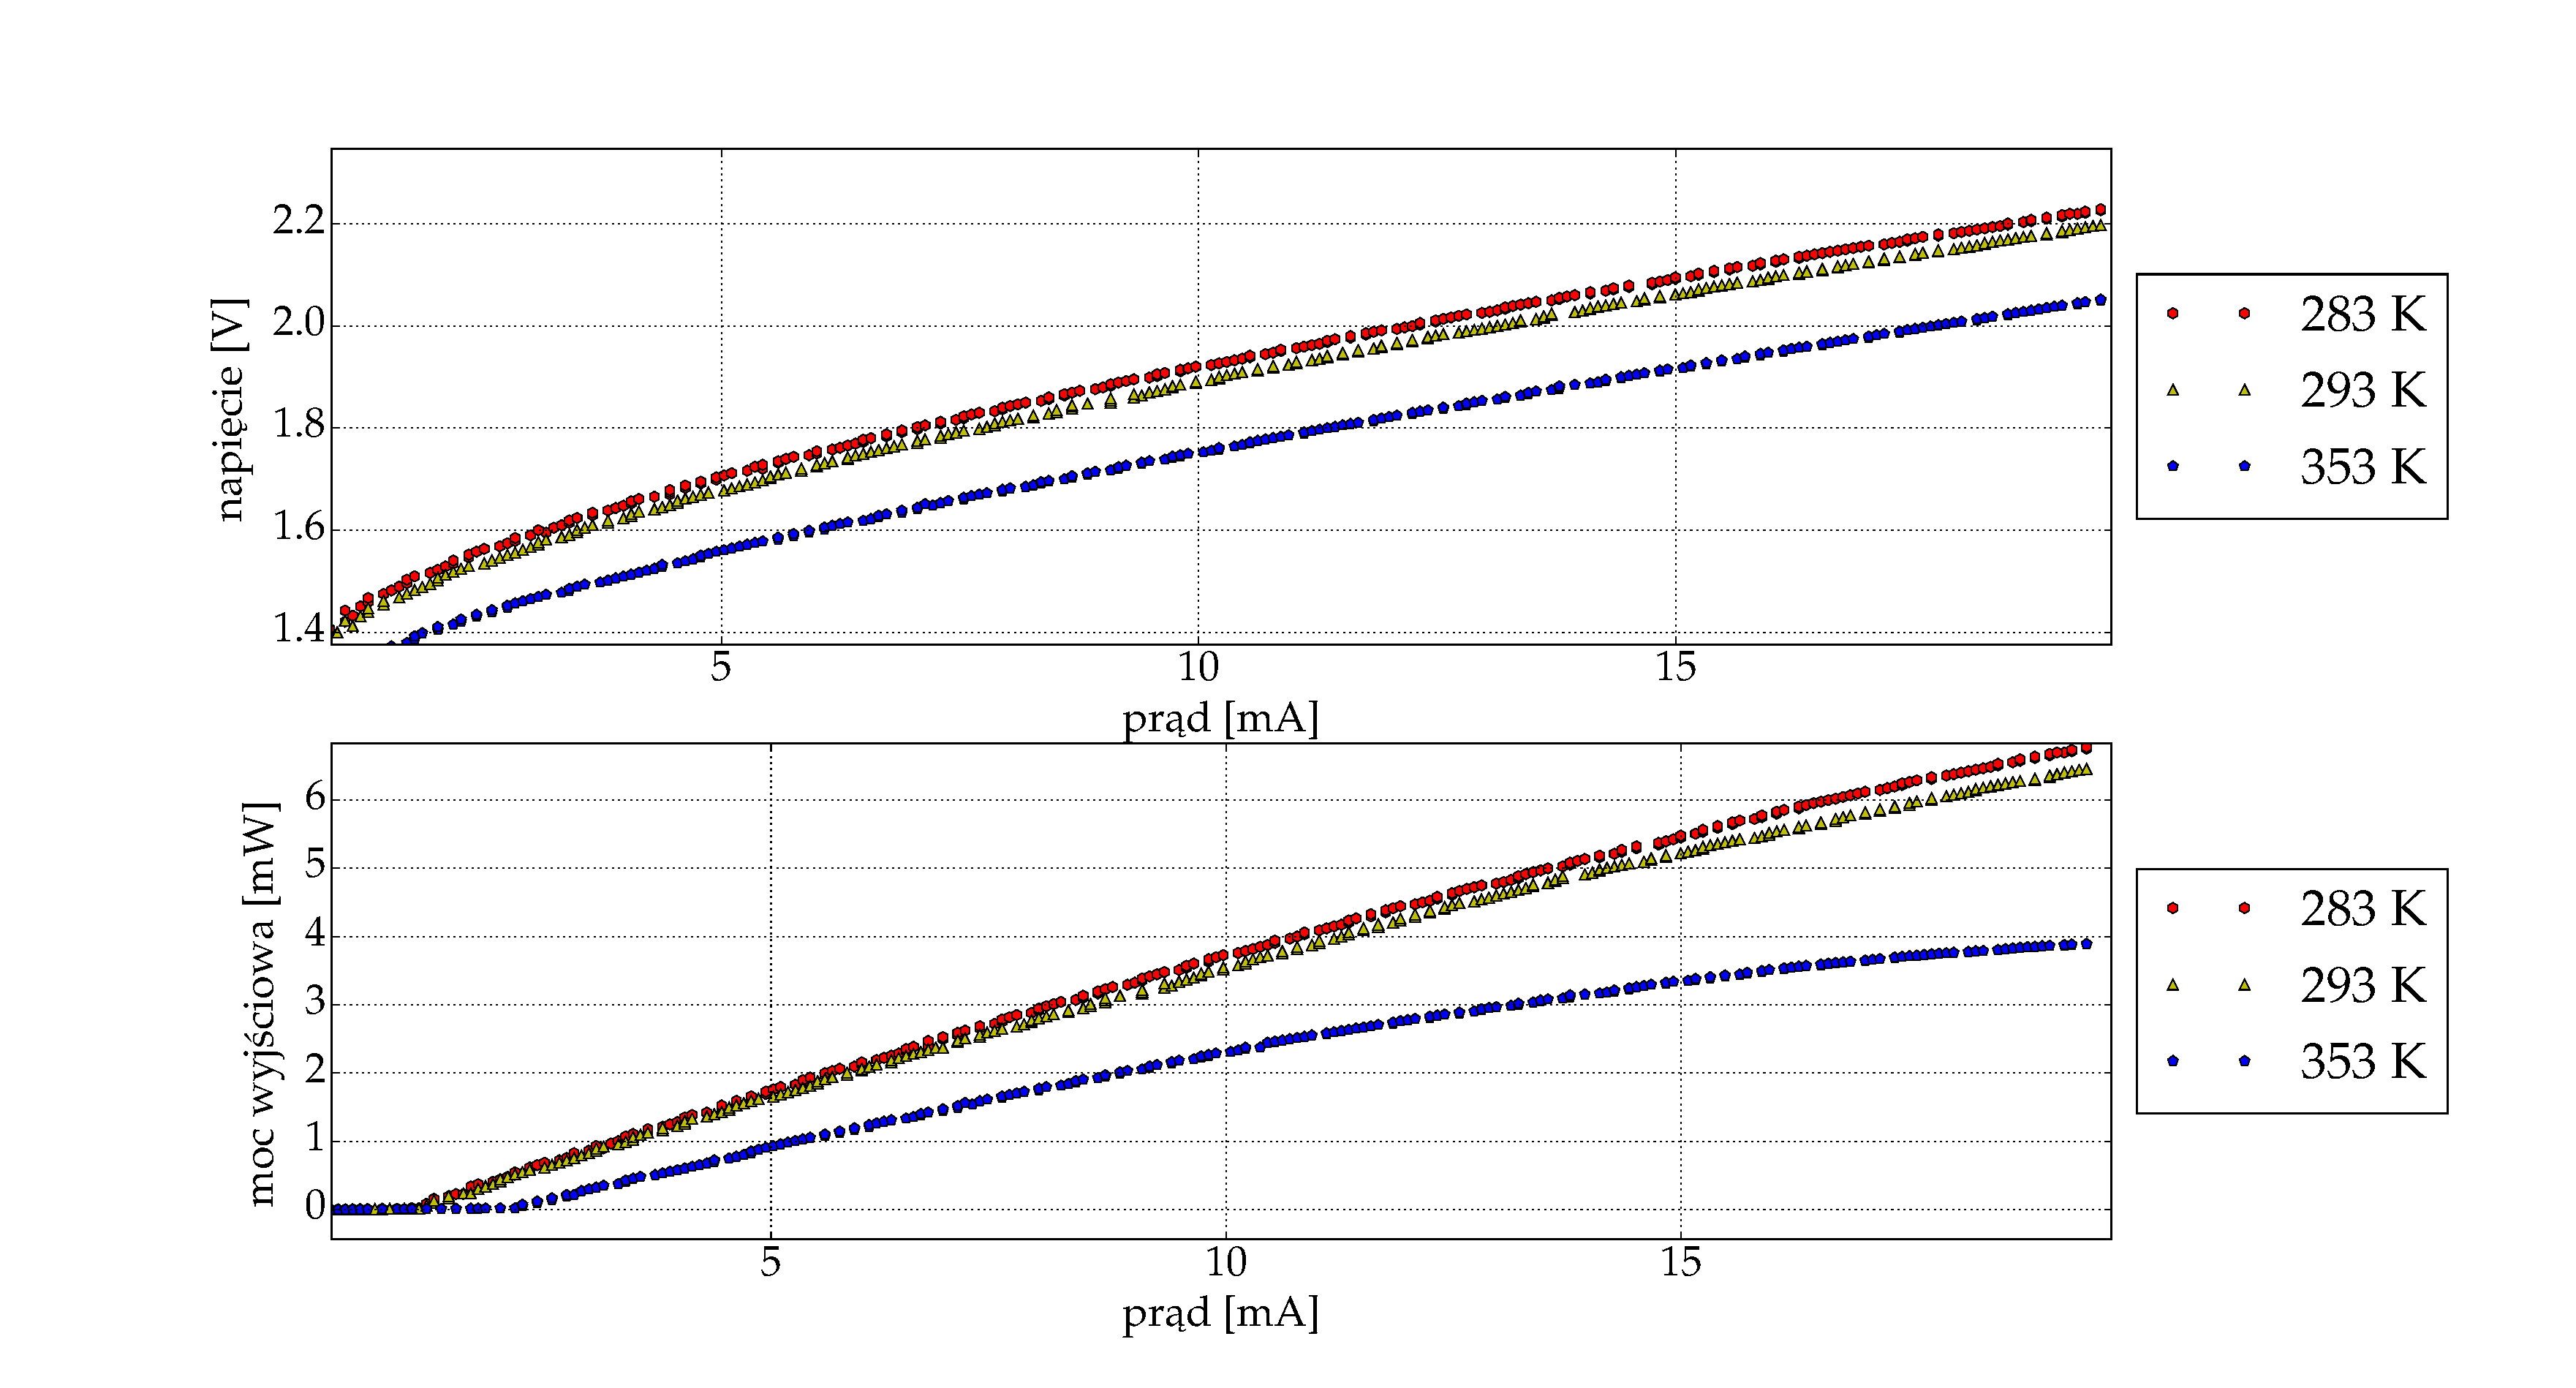
\includegraphics[scale=0.30]{plot980/plot_i_v_i_l.eps}
  \caption{Wykres napięcia oraz mocy wyjściowej w fukcji prądu dla lasera VCSEL 980\,nm.}
  \label{fig:plot_i_v_i_l_980}
\end{figure}
\begin{figure}
\center
  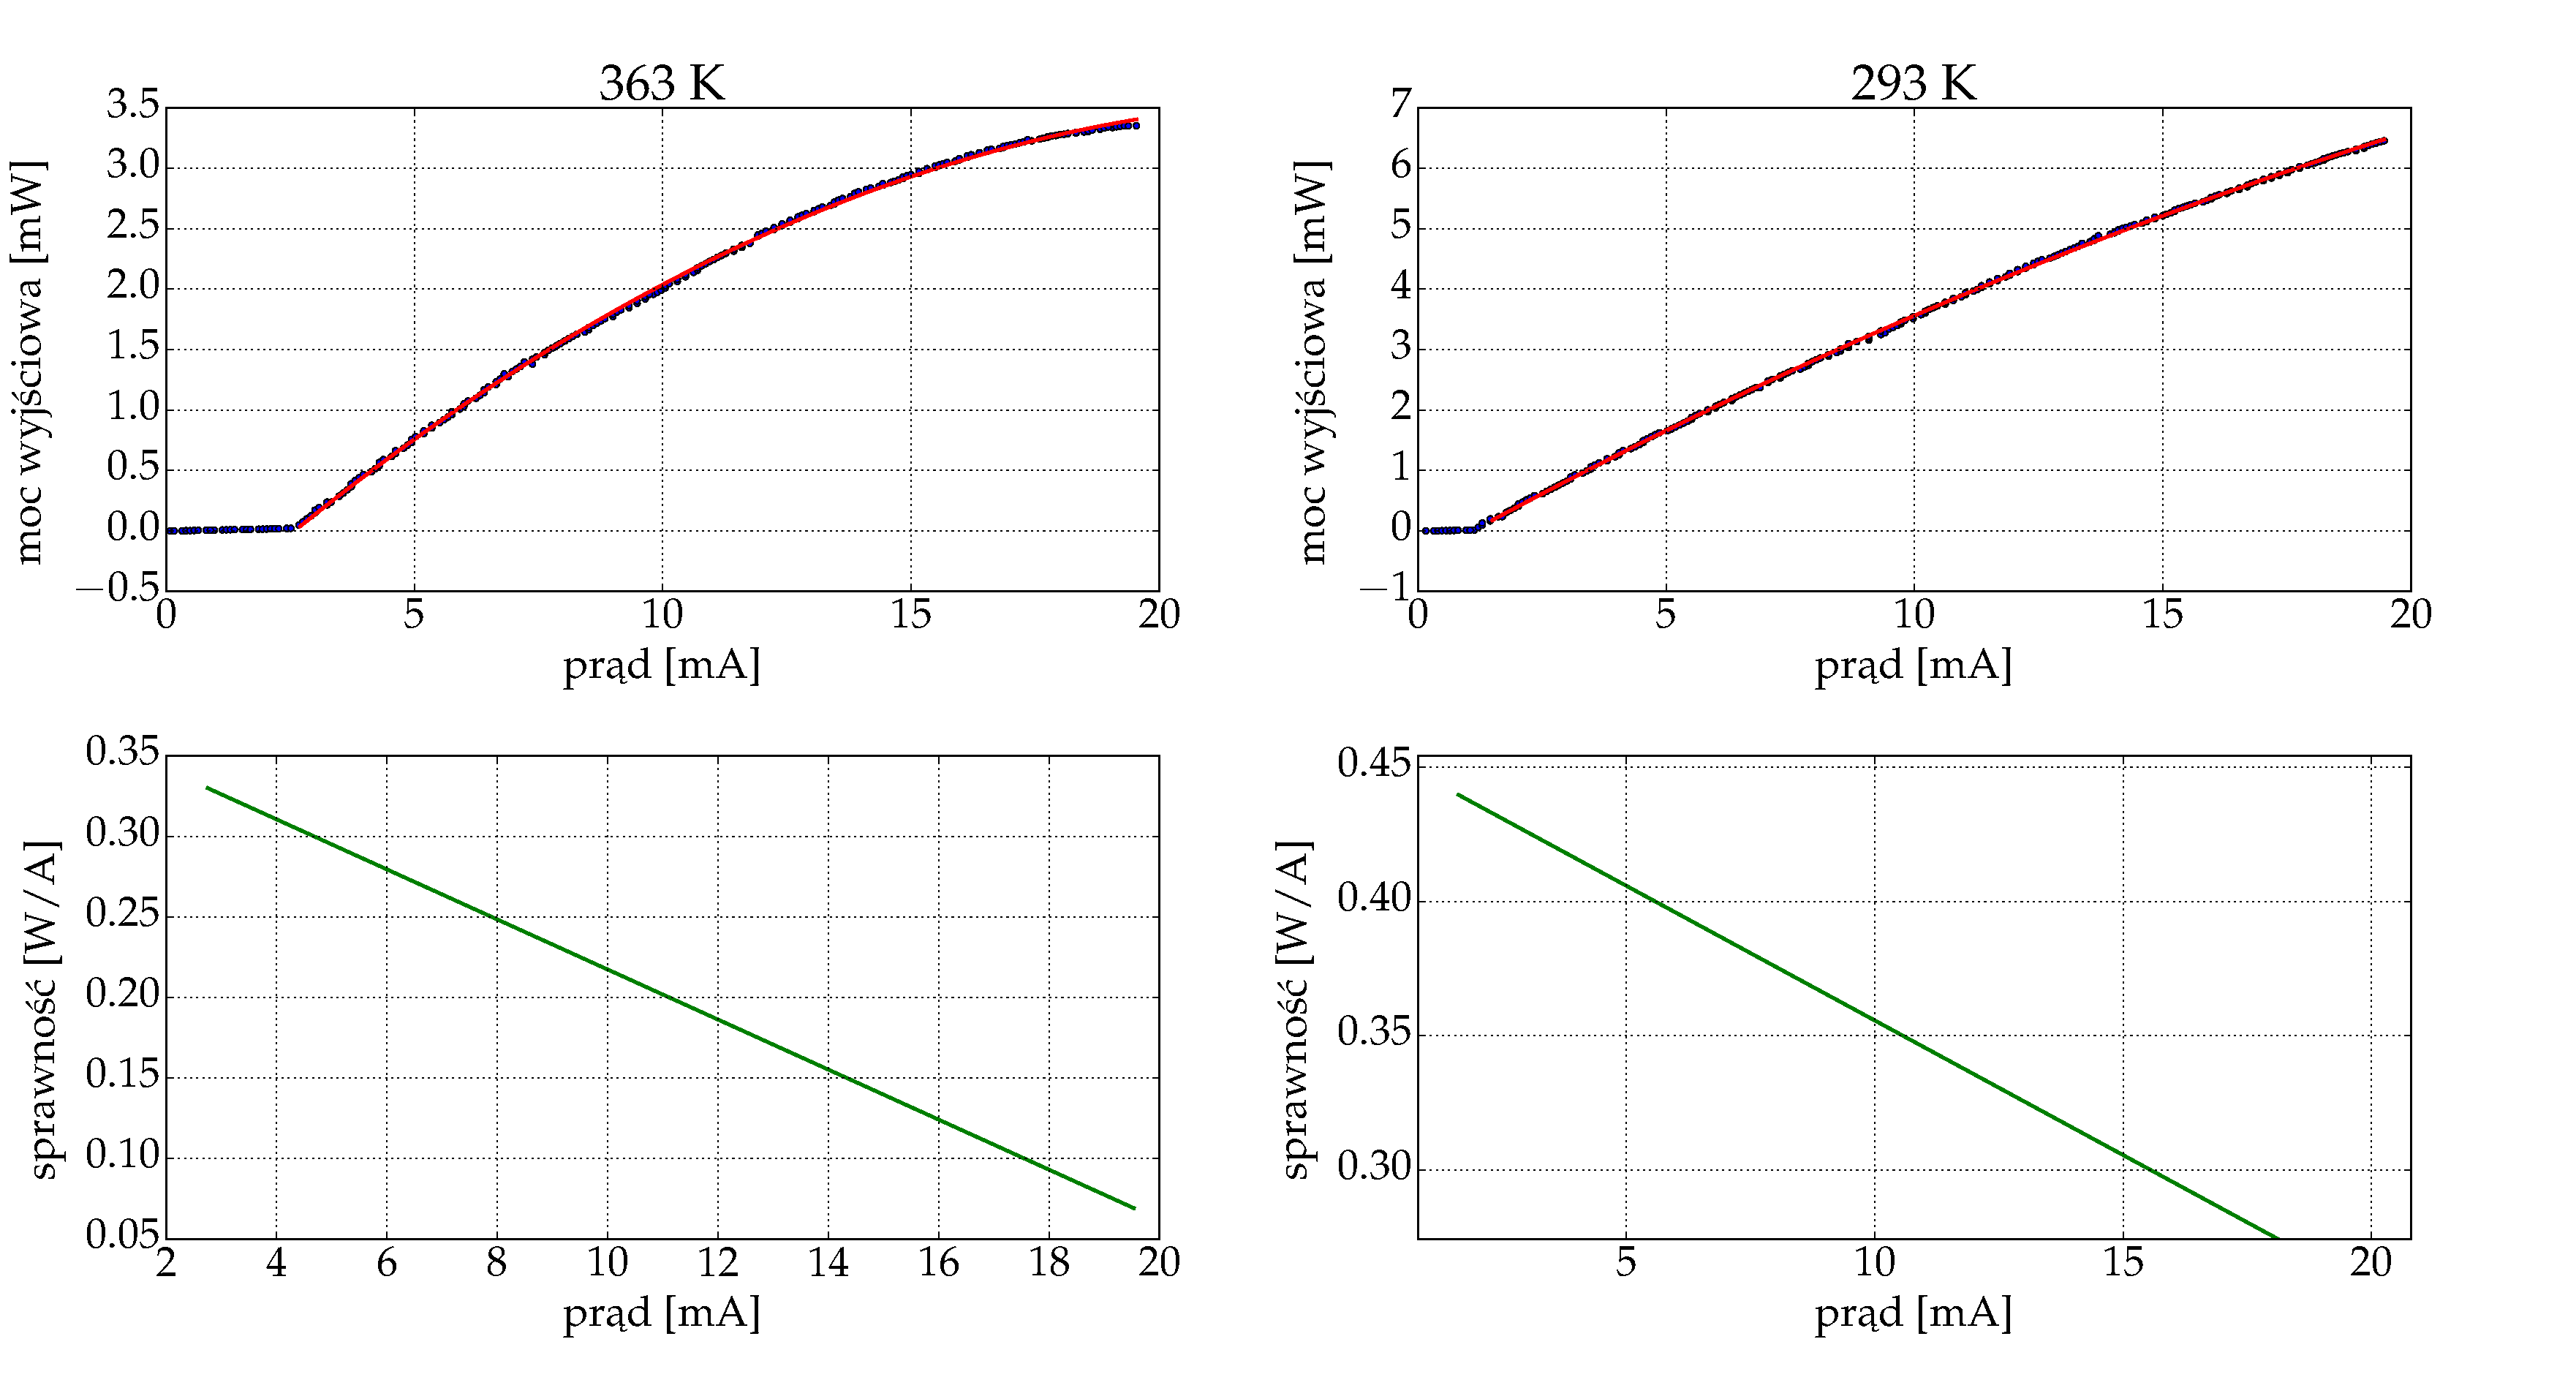
\includegraphics[scale=0.30]{plot980/plot_eff_via_current4.eps}
  \caption{Wykres sprawności różnoczkowej dla lasera VCSEL 980\,nm w dwóch różnych temperaturach.}
  \label{fig:plot_eff_via_current4_980}
\end{figure}
\begin{figure}
\center
  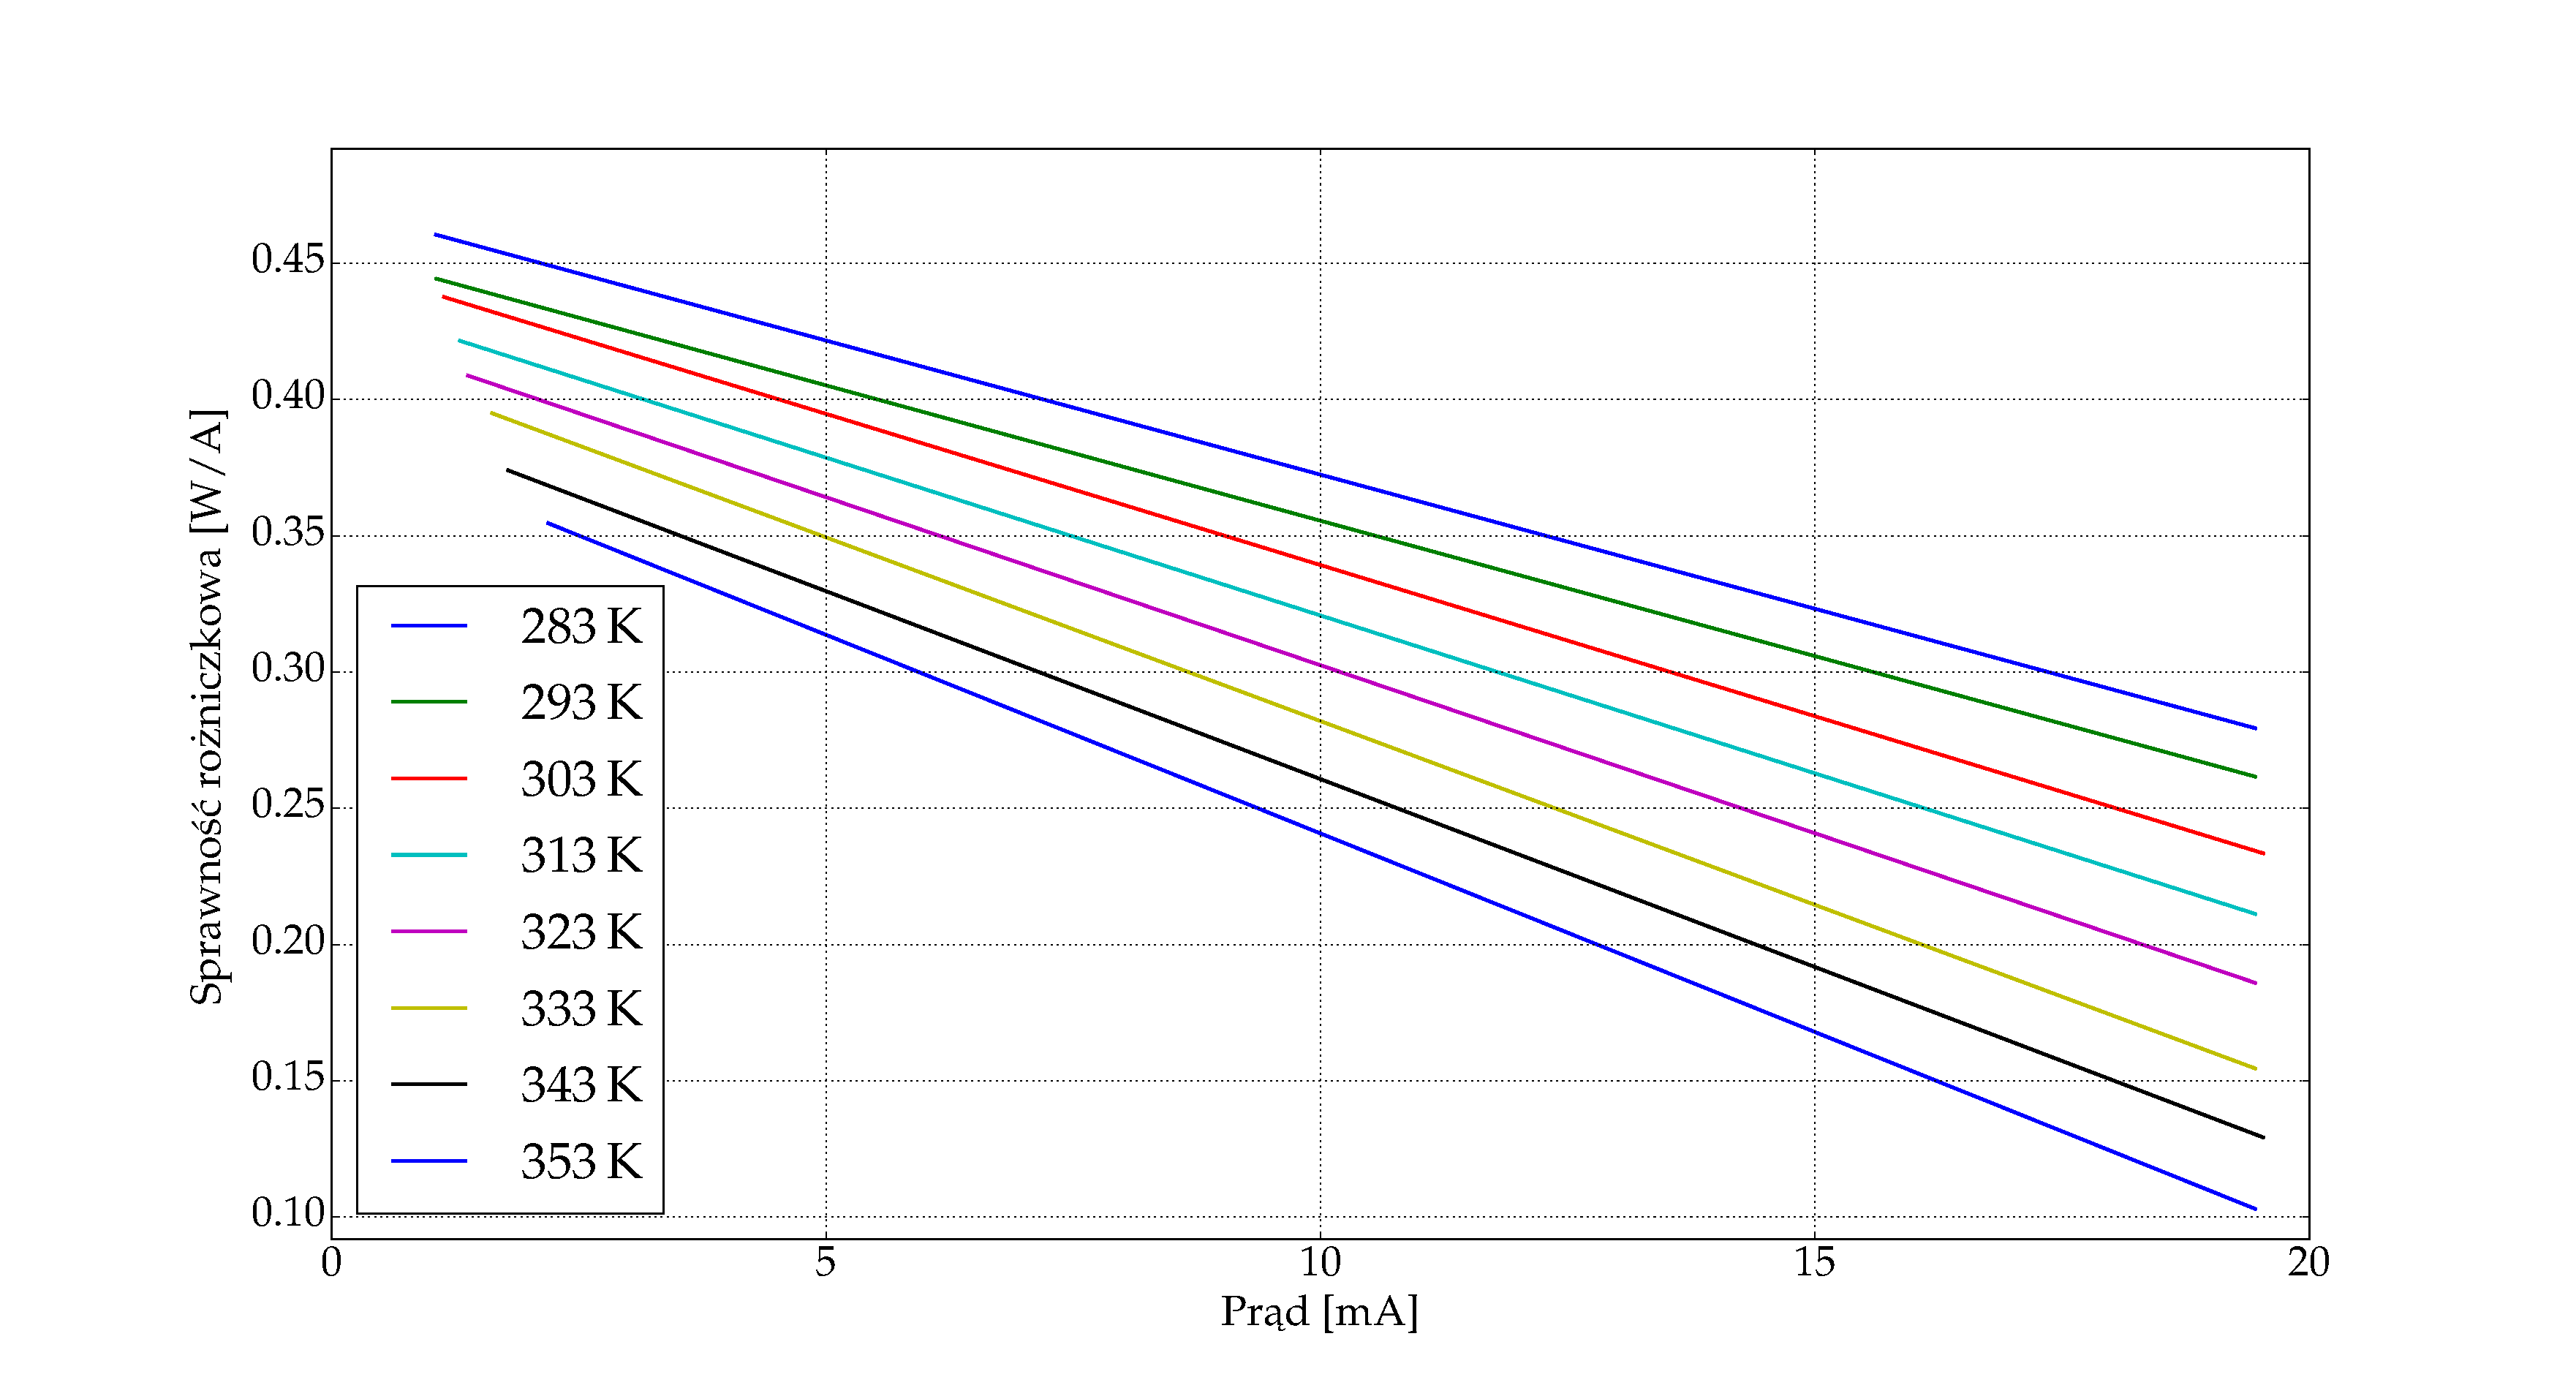
\includegraphics[scale=0.30]{plot980/plot_eff_via_current_all.eps}
  \caption{Wykres sprawności różniczkowej dla lasera VCSEL 980\,nm w różnych temperaturach.}
  \label{fig:plot_eff_via_current_all_980}
\end{figure}